\documentclass[12pt]{article}
\usepackage[left=0.25cm,top=1cm,right=0.25cm,bottom=1cm]{geometry}
\textwidth = 20cm
\hoffset = -1cm
\usepackage[utf8]{inputenc}
\usepackage[spanish,es-tabla]{babel}
\usepackage[autostyle,spanish=mexican]{csquotes}
\usepackage[tbtags]{amsmath}
\usepackage{nccmath}
\usepackage{amsthm}
\usepackage{amssymb}
\usepackage{graphicx}
\usepackage{standalone}
\usepackage[outdir=./]{epstopdf}
\usepackage{siunitx}
\usepackage{physics}
\usepackage{color}
\usepackage{float}
\usepackage{multicol}
%\usepackage{milista}
\usepackage{enumitem}
\usepackage{anyfontsize}
\usepackage{anysize}
\usepackage{enumitem}
\usepackage{capt-of}
\usepackage{bm}
\usepackage{relsize}
\usepackage{placeins}
\usepackage{empheq}
\usepackage{cancel}
\usepackage{wrapfig}
\spanishdecimal{.}
\renewcommand{\baselinestretch}{1.5} 
\renewcommand\labelenumii{\theenumi.{\arabic{enumii}}}
\newcommand{\ptilde}[1]{\ensuremath{{#1}^{\prime}}}
\newcommand{\stilde}[1]{\ensuremath{{#1}^{\prime \prime}}}
\newcommand{\ttilde}[1]{\ensuremath{{#1}^{\prime \prime \prime}}}
\newcommand{\ntilde}[2]{\ensuremath{{#1}^{(#2)}}}



\title{Analizando la parte angular del átomo de hidrógeno \\ {\large Tema 4}\vspace{-3ex}}
\author{M. en C. Gustavo Contreras Mayén}
\date{ }

\pagestyle{fancy}
\fancyhf{}
\rhead{Curso MAF}
\lhead{\leftmark}
\rfoot{\thepage}
\setlength{\headheight}{16pt}%

\def\changemargin#1#2{\list{}{\rightmargin#2\leftmargin#1}\item[]}
\let\endchangemargin=\endlist 


\begin{document}
\maketitle
\fontsize{14}{14}\selectfont
\tableofcontents
\newpage

%Ref. El átomo de hidrógeno
\section{La función de onda.}

De la revisión del problema del átomo de hidrógeno, mediante la técnica de separación de variables, es posible deducir la expresión de la función de onda:
\begin{align}
\psi_{n, \ell, m} (r, \theta, \phi) = R _{n, \ell} (r) \, \Theta_{\ell, m} (\theta) \, \Phi_{m} (\phi)
\label{ec:ecuacion_07_25}
\end{align}
Tendremos esta función de onda para cada terna de números cuánticos que satisfagan las condiciones:
\begin{align}
\begin{aligned}
n &\geq 1 \hspace{0.2cm} n = 1, 2, 3, \ldots \\[0.5em]
\ell &= 0, 1, \ldots, (n - 1) \\[0.5em]
m &= \ell, \ell - 1, \ldots, 0, - \ell + 1, -\ell
\end{aligned}
\label{eq:ecuacion_07_26}
\end{align}
pues en otro caso, no es posible satisfacer las condiciones de frontera. Las funciones de onda del hidrógeno, reciben también el nombre de \emph{orbitales atómicos}.
\par
Por ejemplo, con $n = 2$ veremos cuántas funciones de onda pueden construirse: $\ell$ solo puede tomar los valores $\ell = 0, 1$, en el primer caso $m$ solo puede valer $m = 0$, mientras que para $\ell = 1$, $m = -1, 0, 1$. Es decir, se pueden obtener cuatro funciones de onda:
\begin{align*}
\psi_{2, 0, 0} (r, \theta, \phi) &= R_{2, 0} (r) \, \Theta_{0, 0} (\theta) \, \Phi_{0} (\phi) \\[0.5em]
\psi_{2, 1, 1} (r, \theta, \phi) &= R_{2, 1} (r) \, \Theta_{1, 1} (\theta) \, \Phi_{1} (\phi) \\[0.5em]
\psi_{2, 1, 0} (r, \theta, \phi) &= R_{2, 1} (r) \, \Theta_{1, 0} (\theta) \, \Phi_{0} (\phi) \\[0.5em]
\psi_{2, 1, -1} (r, \theta, \phi) &= R_{2, 1} (r) \, \Theta_{1, -1} (\theta) \, \Phi_{-1} (\phi)
\end{align*}
Encontrar que la función radial de la primera es distinta a las otras tres, que tienen la misma descripción radial.
\par
Podríamos preguntarnos ahora: ¿qué forma adquiere la función radial $R_{2, 1} (r)$ o la función angular $\Theta_{0, 0} (\theta) \, \Phi_{0} (\phi)$ del ejemplo anterior? La respuesta es fácil de dar, lo difícil, es obtenerlas.
\par
A continuación, presentaremos algunas funciones radiales (ver Tabla \ref{table:Tabla_funciones_radiales}) y angulares (Tabla \ref{table:Tabla_funciones_angulares}) para el átomo de hidrógeno (tomaremos prestados los resultados), encontraremos que se incluyen funciones trigonométricas y exponenciales. El valor de $\pderivada{a}_{0}$ es el radio de Bohr calculado con la masa reducida $\mu$, es decir:
\begin{align}
\pderivada{a}_{0} = \dfrac{\hbar^{2}}{\kappa \, \mu \, e^{2}} = a_{0} \, \dfrac{m_{e}}{\mu}
\label{eq:ecuacion_07_27}
\end{align}

\begin{table}[H]
\centering
\large
\renewcommand{\arraystretch}{1.5}
\begin{tabular}{|c | c | c|} \hline
$n$ & $\ell$ & $R_{n, \ell} (r)$ \\ \hline
$1$ & $0$ & $2 \bigg( \dfrac{Z}{\pderivada{a}_{0}} \bigg)^{\frac{3}{2}} \, \exp\bigg( \dfrac{Z r}{2 \pderivada{a}_{0}} \bigg)$ \\ \hline
$2$ & $0$ & $\dfrac{1}{2 \sqrt{2}} \bigg( \dfrac{Z}{\pderivada{a}_{0}} \bigg)^{\frac{3}{2}} \, \bigg( 2 - \dfrac{Z r}{\pderivada{a}_{0}} \bigg) \, \exp\bigg( \dfrac{Z r}{2 \pderivada{a}_{0}} \bigg)$ \\ \hline
$2$ & $1$ & $\dfrac{1}{2 \sqrt{6}} \bigg( \dfrac{Z}{\pderivada{a}_{0}} \bigg)^{\frac{3}{2}} \, \bigg( \dfrac{Z r}{\pderivada{a}_{0}} \bigg) \, \exp\bigg( \dfrac{Z r}{2 \pderivada{a}_{0}} \bigg)$ \\ \hline
$3$ & $0$ & $\dfrac{2}{81 \sqrt{3}} \bigg( \dfrac{Z}{\pderivada{a}_{0}} \bigg)^{\frac{3}{2}} \, \bigg[ 2 \bigg( \dfrac{Z r}{\pderivada{a}_{0}} \bigg)^{2} - 18 \bigg( \dfrac{Z r}{\pderivada{a}_{0}} \bigg) + 27 \bigg] \, \exp\bigg( \dfrac{Z r}{3\pderivada{a}_{0}} \bigg)$ \\ \hline
$3$ & $1$ & $\dfrac{2 \sqrt{2}}{81 \sqrt{3}} \bigg( \dfrac{Z}{\pderivada{a}_{0}} \bigg)^{\frac{3}{2}} \, \bigg[ 6 - 18 \bigg( \dfrac{Z r}{\pderivada{a}_{0}} \bigg) \bigg] \, \exp\bigg( \dfrac{Z r}{3\pderivada{a}_{0}} \bigg)$ \\ \hline
\end{tabular}
\caption{Funciones radiales del hidrógeno.}
\label{table:Tabla_funciones_radiales}
\end{table}

\begin{table}[H]
\centering
\large
\renewcommand{\arraystretch}{1.5}
\begin{tabular}{|c | c | c|} \hline
$\ell$ & $m$ & $\Theta_{\ell, m} (\theta) \, \Phi_{m} (\phi)$ \\ \hline
$0$ & $0$ & $(1/4 \pi)^{\frac{1}{2}}$ \\ \hline
$1$ & $0$ & $(3/4 \pi)^{\frac{1}{2}} \, \cos \theta$ \\ \hline
$1$ & $1$ & $(3/8 \pi)^{\frac{1}{2}} \, \sin \theta e^{i \phi}$ \\ \hline
$1$ & $-1$ & $(3/8 \pi)^{\frac{1}{2}} \, \sin \theta e^{-i \phi}$ \\ \hline
$2$ & $0$ & $(5/16 \pi)^{\frac{1}{2}} \, (3 \, \cos \theta - 1)$ \\ \hline
$2$ & $1$ & $(15/8 \pi)^{\frac{1}{2}} \, \sin \theta \, \cos \theta \, e^{i \phi}$ \\ \hline
$2$ & $-1$ & $(15/8 \pi)^{\frac{1}{2}} \, \sin \theta \, \cos \theta \, e^{-i \phi}$ \\ \hline
\end{tabular}
\caption{Funciones angulares del hidrógeno.}
\label{table:Tabla_funciones_angulares}
\end{table}

\subsection{Notación.}

Se muestra a continuación la notación simbólica que se acostumbra utilizar para denotar a las funciones de onda. Cada una está caracterizada por los números $n, \ell$ y $m$, pero es usual la notación con los valores de $\ell$:
\begin{table}
\centering
\large
\begin{tabular}{|c | c | l|} \hline
$\ell$ & Símbolo & Significado \\ \hline
$0$ & \emph{s} & Sharp (exacta) \\ \hline
$1$ & \emph{p} & Principal (principal) \\ \hline
$2$ & \emph{d} & Difuse (difusa) \\ \hline
$3$ & \emph{f} & Fundamental (fundamental) \\ \hline
$4$ & \emph{g} & Ninguno \\ \hline
$5$ & \emph{h} & Ninguno \\ \hline
\vdots & \vdots & \vdots \\ \hline    
\end{tabular}
\caption{Símbolos para los valores de $\ell$.}
\label{table:Tabla_valores_l}
\end{table}

Cuando se hace referencia a la función $2 p_{1}$, es aquella con $n = 2$, $\ell = 1$ y $m = 1$; cuando se tiene la $3 d_{-2}$, se está definiendo a la función con $n = 3$, $\ell = 2$ y $m = -2$. En el caso de los orbitales $s$, donde $\ell = 0$ y $m$ no tiene otro posible valor más que cero, se evita el subíndice que especifica $m$. Por lo que, el orbital $4s$ será aquel con $n = 4$, $\ell = 0$ y $m = 0$.

\section{Análisis de la parte angular.}

Es de mucho interés extraer toda la información posible de la función de onda del átomo de hidrógeno. Entre otras cosas, se puede analizar la densidad de la probabilidad para el electrón y los valores precisos o promedio de otras variables, como la distancia al núcleo, el momento angular, la energía cinética, etc.
\par
Consideremos el cuadrado de la función de onda, por lo que la densidad de probabilidad $\rho (r, \theta, \phi)$ es:
\begin{align}
\begin{aligned}[b]
\rho (r, \theta, \phi) &= \abs{\psi_{n, \ell, m} (r, \theta, \phi)}^{2} = \\[0.5em]
&= R_{n,\ell}^{2} (r) \, \Theta_{\ell,m}^{2} (\theta) \abs{\Phi_{m} (\phi)}^{2}
\end{aligned}
\label{eq:ecuacion_07_42}
\end{align}
Se revisará inicialmente la parte angular, es decir: $\Theta_{\ell,m}^{2} (\theta) \abs{\Phi_{m} (\phi)}^{2}$.
\par
A la función:
\begin{align}
Y_{\ell, m} = \Theta_{\ell,m} (\theta) \,\Phi_{m} (\phi)
\label{eq:ecuacion_07_76}
\end{align}
le llamaremos \textbf{\textcolor{blue}{armónico esférico}}. La componente $\phi$ de los armónicos esféricos es una función compleja, ya que como se revisa en la Tabla (\ref{table:Tabla_funciones_angulares}), contiene factores del tipo $e^{i m \phi}$. Sin embargo, se puede demostrar cómo con una combinación adecuada de los armónicos esféricos, se producen solamente funciones de valor real, conocidas como \textbf{\textcolor{red}{armónicos esféricos reales}}.

\subsection{Armónicos esféricos reales.}

Si queremos graficar en coordenadas polares las partes angulares de los orbitales del hidrógeno (Tabla \ref{table:Tabla_funciones_angulares}), se presenta un grave problema: la función $\Phi_{m} (\phi) = (1/2 \pi)^{\frac{1}{2}} \, e^{i m \phi}$ toma valores complejos. Mientras $m = 0$, no hay problema alguno, pero si el valor no es cero, no queda claro cómo graficar sobre la coordenada $r$ una distancia compleja.
\par
Las partes real e imaginaria de estas funciones, se recuperan con la identidad de Euler:
\begin{align}
e^{i m \phi} = \cos m \phi + i \, \sin m \phi
\label{eq:ecuacion_07_79}
\end{align}
Una manera de evitar los números complejos es trabajar con el módulo de los mismos, que es un número real. Por lo tanto, el módulo de la ec. (\ref{eq:ecuacion_07_79}), es:
\begin{align}
\abs{e^{i m \phi}} = \sqrt{ \cos^{2} m \phi + \sin^{2} m \phi} = 1
\label{eq:ecuacion_07_80}
\end{align}

Las primeras funciones donde aparece $m \neq 0$ son la $p_{+1}$ y la $p_{-1}$ que, al revisar los valores de la Tabla (\ref{table:Tabla_funciones_angulares}), son:
\begin{align}
Y_{1, 1} (\theta, \phi) &= \bigg( \dfrac{3}{8} \bigg)^{\frac{1}{2}} \, \sin \theta \, e^{i \phi} \label{eq:ecuacion_07_81} \\[0.5em]
Y_{1, -1} (\theta, \phi) &= \bigg( \dfrac{3}{8} \bigg)^{\frac{1}{2}} \, \sin \theta \, e^{-i \phi} \label{eq:ecuacion_07_82}
\end{align}
Ocupando la ec. (\ref{eq:ecuacion_07_80}), el módulo de ambas funciones es idéntico:
\begin{align}
\abs{Y_{1, 1} (\theta, \phi)} = \abs{Y_{1, -1} (\theta, \phi)} = \bigg( \dfrac{3}{8} \bigg)^{\frac{1}{2}} \, \sin \theta
\label{eq:ecuacion_07_83}
\end{align}
Un esbozo de la gráfica de esta función en coordenadas polares se muestra en la figura (\ref{fig:figura_plot_Y11_01}):
\begin{figure}[H]
    \centering
    \includegraphics[scale=0.75]{Imagenes/Plot_Y11_01.eps}
    \caption{Gráfica del $\abs{Y_{1, 1} (\theta, \phi)}$ en el plano.}
    \label{fig:figura_plot_Y11_01}
\end{figure}
En la figura (\ref{fig:figura_plot_Y11_02}) se presenta la misma función, pero ahora al graficarla en el espacio:
\begin{figure}[H]
    \centering
    \includegraphics[scale=1]{Imagenes/Plot_Y11_02.eps}
    \caption{Gráfica del $\abs{Y_{1, 1} (\theta, \phi)}$ en el espacio.}
    \label{fig:figura_plot_Y11_02}
\end{figure}

Como se ve, al tomar el módulo se ha perdido información de la función de onda, ya que no se puede diferenciar entre $p_{+1}$ y $p_{-1}$. Sin embargo, como lo que interesa en realidad es el cuadrado de la función de onda, y como los cuadrados de las ecs. (\ref{eq:ecuacion_07_81}) y (\ref{eq:ecuacion_07_82}) son iguales al de la función módulo, ec. (\ref{eq:ecuacion_07_83}), ésta última resulta de utilidad.
\par
Se acostumbra analizar las partes angulares haciendo combinaciones de las funciones complejas con objeto de obtener funciones de valor real. Para ello se aprovechan las siguientes identidades:
\begin{align}
\cos m \phi &= \dfrac{e^{i m \phi} + e^{-i m \phi}}{2} \label{eq:ecuacion_07_84} \\[0.5em]
\sin m \phi &= \dfrac{e^{i m \phi} - e^{-i m \phi}}{2 \, i} \label{eq:ecuacion_07_85}
\end{align}
Por ejemplo, las siguientes combinaciones de las funciones $p_{+1}$ y $p_{-1}$, resultan ser funciones de valor real\footnote{Los factores $2$ se introducen para que las nuevas funciones cumplan con la condición de normalización.}:
\begin{align}
Y_{1, \cos}^{1} (\theta, \phi) &= \dfrac{Y_{1,1} (\theta, \phi) + Y_{1, -1} (\theta, \phi)}{\sqrt{2}} \label{eq:ecuacion_07_86} \\[0.5em]
Y_{1, \sin}^{1} (\theta, \phi) &= \dfrac{Y_{1,1} (\theta, \phi) - Y_{1, -1} (\theta, \phi)}{\sqrt{2}} \label{eq:ecuacion_07_87}
\end{align}
Estos resultados se demuestran fácilmente al sustituir las ecs. (\ref{eq:ecuacion_07_81}) y (\ref{eq:ecuacion_07_82}) en las ecs. (\ref{eq:ecuacion_07_86}) y (\ref{eq:ecuacion_07_87}), ocupando las relaciones (\ref{eq:ecuacion_07_84}) y (\ref{eq:ecuacion_07_85}) para $m = 1$, de donde se obtiene:
\begin{align}
Y_{1, \cos}^{1} (\theta, \phi) &= \bigg( \dfrac{3}{4} \bigg)^{\frac{1}{2}} \sin \theta \cos \phi \label{eq:ecuacion_07_88} \\[0.5em]
Y_{1, \sin}^{1} (\theta, \phi) &= \bigg( \dfrac{3}{4} \bigg)^{\frac{1}{2}} \sin \theta \sin \phi \label{eq:ecuacion_07_89}
\end{align}
quedando claro el por qué se eligieron los subíndices \emph{cos} y \emph{sin} para estas nuevas funciones. Los superíndices $1$ se refieren a $\abs{m}$.
\par
Los armónicos esféricos obtenidos por este procedimiento se conocen como \textbf{\textit{armónicos esféricos reales}}. El \enquote{precio} que debe de pagarse por haber evitado los números complejos, es que las nuevas funciones no están caracterizadas más que por el número cuántico $\ell$ y la paridad (seno o coseno) de la función $\phi$. Se ha perdido el número cuántico $m$, pues los armónicos esféricos reales se obtienen por combinaciones entre dos soluciones con diferentes valores de $m$. Sólo corresponden a un valor de $\abs{m}$.

\subsection{Nombres nuevos a los AER.}

Los armónicos esféricos reales (AER) reciben un nombre por la forma que adquieren al ser expresados en coordenadas cartesianas. De la relación:
\begin{align*}
x &= r \, \sin \theta \, \cos \phi \\[0.5em]
\sin \theta \, \cos \phi &= \dfrac{x}{r}
\end{align*}
la ec. (\ref{eq:ecuacion_07_88}) puede escribirse como:
\begin{align*}
Y_{1, \cos}^{1} (\theta, \phi) = \bigg( \dfrac{3}{4} \bigg)^{\frac{1}{2}} \, \dfrac{x}{r}
\end{align*}

Es claro que la función $p$ con paridad par (coseno) toma valores, en cada punto del espacio $(x, y, z)$, directamente proporcionales a su distancia al origen. De aquí que se le conozca como función angular $p_{x}$.
\par
En la Tabla (\ref{table:Tabla_AERN}) se muestran los armónicos esféricos reales $s, p$ y $d$. Puede verse que las funciones con $m = 0$ $(s, p_{z}$ y $d_{z^{2}})$ no se han alterado respecto a la Tabla (\ref{table:Tabla_funciones_angulares}), ya que son de valor real. Todas las demás pueden obtenerse por combinaciones similares a las aplicadas a las funciones $p$ en las ecs. (\ref{eq:ecuacion_07_86}) y (\ref{eq:ecuacion_07_87}).
\begin{table}[H]
\centering
\large
\renewcommand{\arraystretch}{1.5}
\begin{tabular}{|c | c | l|} \hline
 & Nombre & Función \\ \hline
$Y_{0,0}$ & $s$ & $(1/4 \pi)^{\frac{1}{2}}$ \\ \hline
$Y_{1,0}$ & $p_{z}$ & $(3/4 \pi)^{\frac{1}{2}} \cos \theta$ \\ \hline
$Y_{1, \cos}^{1}$ & $p_{x}$ & $(3/4 \pi)^{\frac{1}{2}} \sin \theta \, \cos \phi$ \\ \hline
$Y_{1, \sin}^{1}$ & $p_{y}$ & $(3/4 \pi)^{\frac{1}{2}} \sin \theta \, \sin \phi$ \\ \hline
$Y_{2, 0}$ & $d_{z^{2}}$ & $(5/16 \pi)^{\frac{1}{2}} (3 \cos^{2} \theta  - 1)$ \\ \hline
$Y_{2, \cos}^{1}$ & $d_{xz}$ & $(15/4 \pi)^{\frac{1}{2}} \, \sin \theta \, \cos \theta \, \cos \phi$ \\ \hline
$Y_{2, \sin}^{1}$ & $d_{yz}$ & $(15/4 \pi)^{\frac{1}{2}} \, \sin \theta \, \cos \theta \, \sin \phi$ \\ \hline
$Y_{2, \cos}^{2}$ & $d_{x^{2}-y^{2}}$ & $(15/16 \pi)^{\frac{1}{2}} \, \sin^{2} \theta \, \cos 2 \theta$ \\ \hline
$Y_{2, \sin}^{2}$ & $d_{xy}$ & $(15/16 \pi)^{\frac{1}{2}} \, \sin^{2} \theta \, \sin 2 \theta$ \\ \hline
\end{tabular}
\caption{Armónicos esféricos reales normalizados.}
\label{table:Tabla_AERN}
\end{table}

\subsection{Gráfica de los AER.}

\subsection*{Las funciones \texorpdfstring{$s$}{s}.}

Las funciones $s$, como se puede ver de la Tabla (\ref{table:Tabla_AERN}), son funciones constantes. Para cualquier dirección especificada por los ángulos $\theta$ y $\phi$, la función siempre vale $(4 \pi)^{-\frac{1}{2}} = 0.282$:
\begin{align*}
Y_{0, 0} = 0.282
\end{align*}
Por lo que su gráfica en coordenadas esféricas polares es una esfera, como se ve en la figura (\ref{fig:figura_plot_Y00}).
\begin{figure}[H]
    \centering
    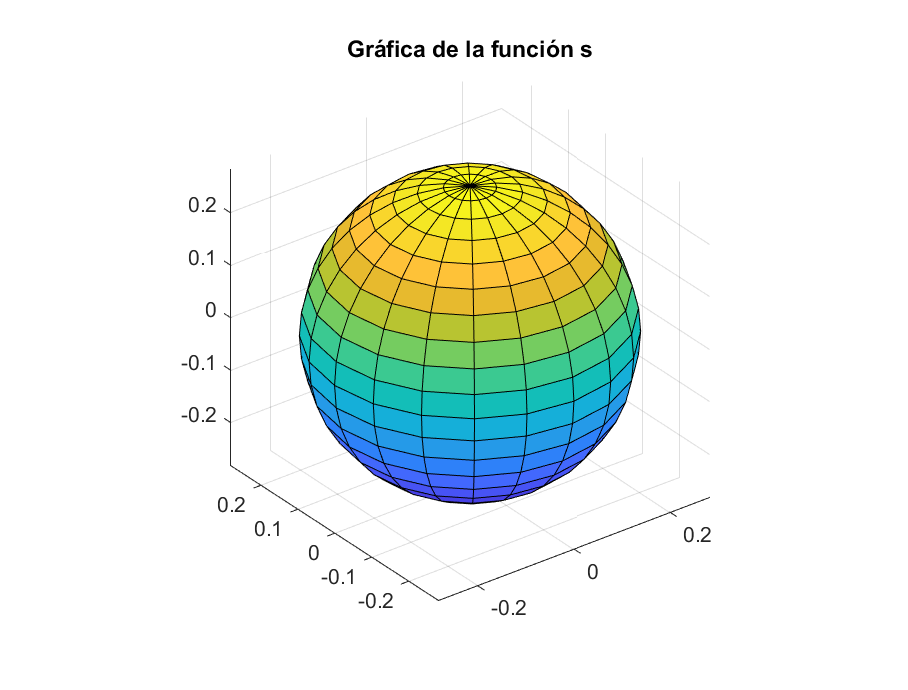
\includegraphics[scale=1]{Imagenes/Plot_Y00_Esfera.eps}
    \caption{Gráfica del AER $Y_{0,0}$ en coordenadas esféricas polares.}
    \label{fig:figura_plot_Y00}
\end{figure}
El cuadrado de esta función representa la contribución de la parte angular del orbital en la densidad de probabilidad. Pero como $[Y_{0,0}]^{2} = 0.076$ es también una constante, su gráfica es asimismo una esfera. Lo que indica que \emph{la densidad de probabilidad de encontrar electrones es la misma independientemente de la dirección que se desee tomar (a partir del núcleo)}.

\subsection*{Las funciones \texorpdfstring{$p$}{p}.}

Nuevamente de la tabla (\ref{table:Tabla_AERN}) podemos reconocer que el factor de normalización:
\begin{align*}
A = (3/4 \pi)^{\frac{1}{2}} = 0.4886
\end{align*}
es el mismo para los tres armónicos esféricos tipo $p$. Sin embargo, su dependencia angular resulta ser diferente, veremos que las tres funciones son equivalentes.
\par
El orbital $p_{z}$ es la función:
\begin{align*}
p_{z} = 0.4886 \, \cos \theta
\end{align*}
Si graficamos la función coseno con el factor de normalización $A$, se tiene lo siguiente:
\begin{figure}[H]
    \centering
    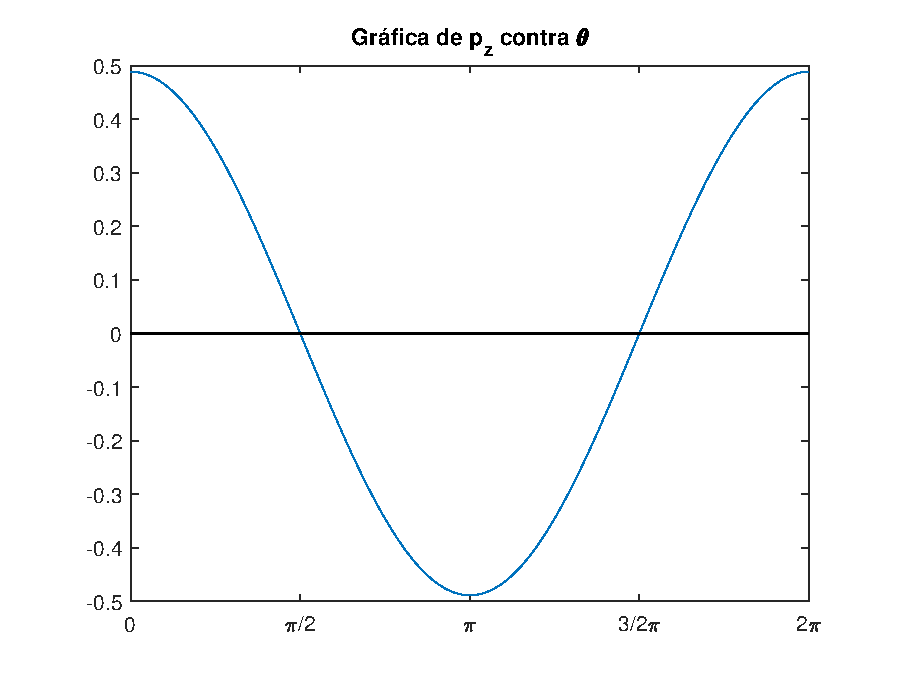
\includegraphics[scale=0.75]{Imagenes/Plot_AER_pz_theta.eps}
    \caption{Gráfica de la función $p_{z}$ contra el ángulo $\theta$.}
    \label{fig:plot_figura_pz_thetha}
\end{figure}
Los valores de la función se representan como una distancia vertical, puede verse que la función toma valores negativos entre $\pi/2$ y $3 \pi/2$ y que su valor máximo ocurre en $\theta = \SI{0}{\degree}$.
\par
Ahora graficamos $p_{z}$ en coordenadas esféricas polares sobre el plano $x-z$, incorporando la gráfica del cuadrado de $p_{z}$.
\par
El plano $x-z$ está compuesto por los dos hemiplanos con $\phi = \SI{0}{\degree}$ y $\phi = \SI{180}{\degree}$. En cada uno de ellos hay que graficar midiendo a partir del eje $z$. Al realizar esta tarea, tenemos la siguiente figura:
\begin{figure}[H]
    \centering
    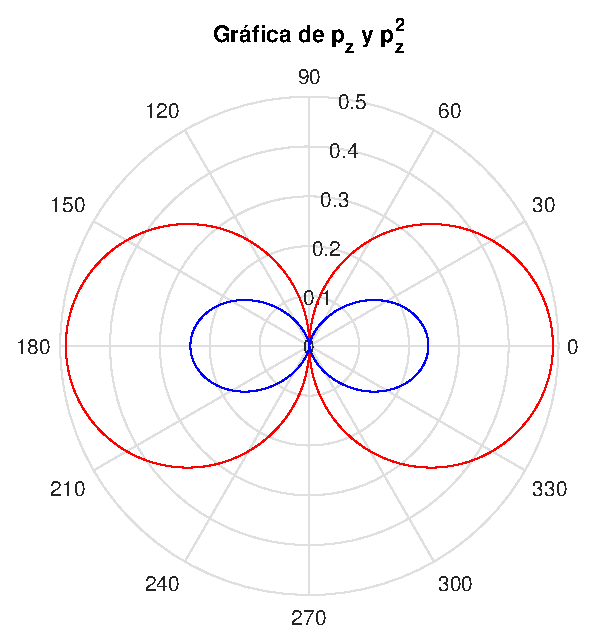
\includegraphics[scale=1]{Imagenes/Plot_AER_pz_theta_pz.eps}
    \caption{Gráfica en coordenadas polares de $p_{z}$ y $p_{z}^{2}$ contra $\theta$.}
    \label{fig:figura_plot_pz_pz2}
\end{figure}
Notemos que por debajo del eje $x$ $(\theta > \SI{90}{\degree})$, la función $p_{z}$ es negativa, pero como lo que se grafica es su valor absoluto, se pierde esta información. Por ello, \emph{se acostumbra colocar un signo \enquote{más} en la región donde la función es positiva y un \enquote{menos} donde es negativa}. Para $\theta = \SI{90}{\degree}$ (ecuación del plano $x-y$), la función $p_{z}$ se anula, por lo que todo el plano $x-y$ es una superficie nodal. En este caso, para las funciones angulares las superficies nodales son planos.
\par
Mientras que para  la gráfica $p_{z}$ resulta de dos círculos tangentes en el origen, su cuadrado tiene una forma oblonga. Así, la contribución angular a la densidad de probabilidad es mayor sobre las direcciones cercanas al eje $z$ y disminuye al alejarse de é{, hasta anularse en el plano $x-y$.
\par
La función $p_{z}$ es independiente del ángulo $\phi$, lo cual implica que es simétrica alrededor del eje $z$. La gráfica total de $p_{z}$ en coordenadas esféricas polares resulta ser un par de esferas tangentes en el origen colocadas sobre el eje $z$.
\begin{figure}[H]
    \centering
    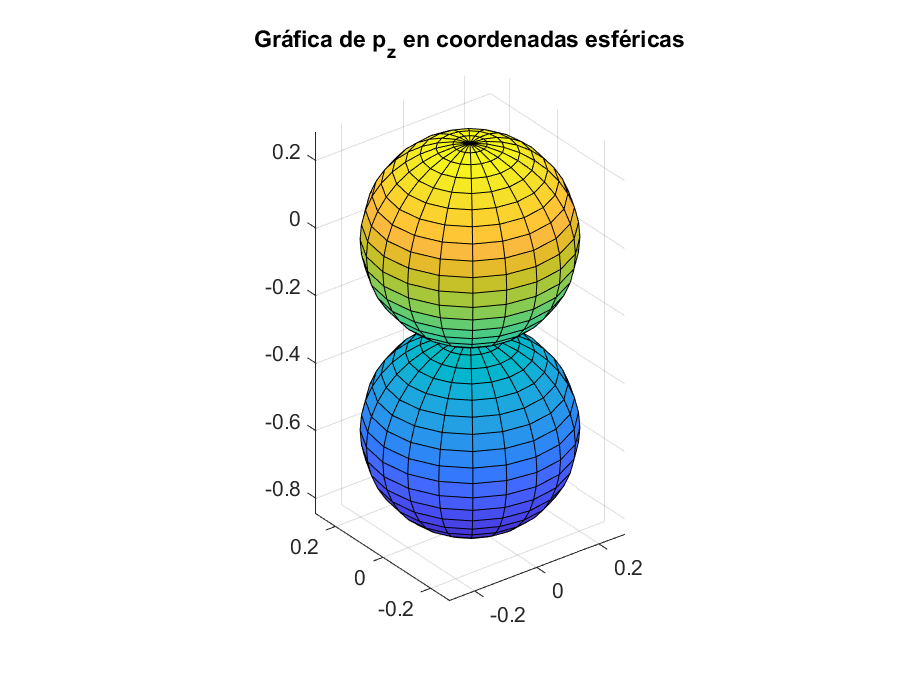
\includegraphics[scale=1]{Imagenes/Plot_AER_pz_theta_total3D.eps}
\end{figure}
Las gráficas correspondientes a los orbitales $p_{x}$ y $p_{y}$ son equivalentes a la de $p_{z}$, con la diferencia de que las esferas están ahora colocadas sobre el eje $x$ y el eje $y$, respectivamente.
\par
En la siguiente figura se presenta el armónico esférico $Y_{1,0} (\theta, \phi)$ que se recupera mediante Mathematica; el análisis que hemos presentado, nos da mucha más información que escribir un script y generar la figura.
\begin{figure}[H]
    \centering
    \includegraphics[scale=1]{Imagenes/Armonicos_Esfericos_10.eps}
\end{figure}
\end{document}